\documentclass{article}


\usepackage{arxiv}

\usepackage[utf8]{inputenc} % allow utf-8 input
\usepackage[T1]{fontenc}    % use 8-bit T1 fonts
\usepackage{hyperref}       % hyperlinks
\usepackage{url}            % simple URL typesetting
\usepackage{booktabs}       % professional-quality tables
\usepackage{amsfonts}       % blackboard math symbols
\usepackage{nicefrac}       % compact symbols for 1/2, etc.
\usepackage{microtype}      % microtypography
\usepackage{lipsum}
\usepackage{graphicx}
\usepackage{subcaption}
\usepackage[margin=1in]{geometry}
\usepackage{amsmath}
\usepackage[spanish]{babel}
\usepackage{float}
\usepackage{adjustbox}
\graphicspath{ {./images/} }
\renewcommand{\refname}{Referencias}


\title{TP 1.1 - SIMULACIÓN DE UNA RULETA}


\author{
 Aldana Risso Patrón \\
  Universidad Tecnológica Nacional - FRRO \\
  Zeballos 1341, S2000, Argentina \\
  \texttt{rissopatronaldana7@gmail.com} \\
   \And
 Ignacio Fierro \\
  Universidad Tecnológica Nacional - FRRO \\
  Zeballos 1341, S2000, Argentina \\
  \texttt{nachofier@gmail.com} \\
  \And
 Lucía Gelmetti \\
  Universidad Tecnológica Nacional - FRRO \\
  Zeballos 1341, S2000, Argentina \\
  \texttt{luligelmetti@gmail.com} \\
  \And
 Juan Cruz Bonanno \\
  Universidad Tecnológica Nacional - FRRO \\
  Zeballos 1341, S2000, Argentina \\
  \texttt{bonanno2340@gmail.com} \\
  \And
 Franco Reggiardo Chuglar \\
  Universidad Tecnológica Nacional - FRRO\\
  Zeballos 1341, S2000, Argentina \\
  \texttt{francoreggiardo15@gmail.com} \\
  \And
 Marcos Oldani \\
  Universidad Tecnológica Nacional - FRRO \\
  Zeballos 1341, S2000, Argentina \\
  \texttt{marcosoldani1360@gmail.com} \\
}

\begin{document}
\maketitle
\begin{abstract}
En este informe se presenta un análisis de los resultados obtenidos a partir de la simulación de la ruleta europea de casino, cuyos números van del 0 al 36, utilizando un programa desarrollado en Python 3.x. A través de múltiples corridas y con un tamaño muestral significativo, se realizó un estudio respaldado por conceptos de Probabilidad y Estadística, complementado con representaciones gráficas de los datos simulados. 
\end{abstract}

\section{Introducción}
Este trabajo práctico tiene como objetivo simular mediante Python el comportamiento estadístico de una ruleta, permitiendo analizar conceptos de probabilidad, la frecuencia relativa, la varianza y la distribución de los resultados.
 A través de múltiples corridas y tiradas, se busca observar cómo se comporta el número elegido frente a la probabilidad teórica, y visualizar estos datos mediante gráficos generados con Matplotlib. Además, se incorporan herramientas de análisis estadístico y visualización para interpretar los resultados de forma clara y fundamentada.

\section {Metodología}

\par Para el desarrollo de este programa, empleamos varias librerías del lenguaje Python, entre las cuales se destacan ``\textit{numpy}'' que se utiliza para el cálculo numérico y el análisis de datos, ``\textit{matplotlib}'' que permite crear y personalizar gráficos en dos dimensiones, ``\textit{sys}'' para la gestión de argumentos en la línea de comandos, y ``\textit{getopt}'' para procesar las opciones ingresadas por la línea de comandos. 

\par La simulación consistirá en realizar n corridas de la ruleta con m tiradas, seleccionando el número x para evaluar su comportamiento. En cada una de las corridas, se calcularán la varianza, desvío estándar, promedio y frecuencia relativa del número x, proporcionando así un análisis detallado de su distribución y comportamiento en el contexto del juego de azar simulado.

\section{Marco Teórico}
\subsection{Definiciones Básicas de Probabilidad y Estadística}
\par Para la buena comprensión del informe, se presentan a continuación una serie de definiciones necesarias:
\begin{itemize}
    \item \textbf{Estadística:} la Estadística se puede comprender como ``el arte de aprender a partir de los datos. Está relacionada con la recopilación de datos, su descripción subsiguiente y su análisis, lo que nos lleva a extraer conclusiones''.
    \item \textbf{Población:} es el grupo o colectivo que se estudia. Este término cuenta aquí con un significado más amplio que en su uso habitual, ya que, se puede referir a personas, cosas o medidas abstractas como el tiempo.
    \item \textbf{Muestra:} cuando se conoce la característica que se quiere estudiar y se ha delimitado la población de estudio, se procede a observar los elementos para obtener la información necesaria.
\end{itemize}

\subsection{Ruleta europea vs. ruleta americana}

\paragraph{Diferencias estructurales.}
Existen dos versiones principales del juego de la ruleta: la \textbf{ruleta europea} y la \textbf{ruleta americana}. Aunque ambas comparten la misma mecánica de juego, presentan diferencias importantes en cuanto a su estructura numérica y, por ende, en sus probabilidades.

La ruleta europea contiene un total de \textbf{37 casillas}, numeradas del 0 al 36. Por otro lado, la ruleta americana incorpora una casilla adicional identificada como \texttt{00}, totalizando \textbf{38 casillas}. Esta diferencia aparentemente menor tiene un impacto significativo en las probabilidades de ganar para el jugador.

\paragraph{Probabilidad de acierto.}
Dado que la apuesta se realiza a un solo número, la probabilidad teórica de acertar dicho número varía entre ambas versiones. En la ruleta europea, esta probabilidad es:

\begin{equation}
    P_{\text{europea}} = \frac{1}{37} \approx 0{,}0270 \quad (2{,}70\%)
\end{equation}

Mientras que en la ruleta americana es:

\begin{equation}
    P_{\text{americana}} = \frac{1}{38} \approx 0{,}0263 \quad (2{,}63\%)
\end{equation}

\paragraph{Ventaja del casino.}
La \textbf{ventaja de la casa} representa el porcentaje del dinero apostado que, en promedio, retiene el casino a largo plazo. Para un juego justo, esta ventaja debería ser nula; sin embargo, las ruletas están diseñadas para que el casino siempre tenga un margen estadístico positivo. En la ruleta europea, dicha ventaja es del 2,70\%, mientras que en la americana asciende al 5,26\% debido a la presencia del doble cero:

\begin{equation}
    \text{Ventaja}_{\text{europea}} = \frac{1}{37} \times 100 \approx 2{,}70\%
\end{equation}

\begin{equation}
    \text{Ventaja}_{\text{americana}} = \frac{2}{38} \times 100 \approx 5{,}26\%
\end{equation}

\paragraph{Elección de tipo de ruleta para la simulación.}
Dado que la ruleta europea ofrece una menor ventaja al casino y es la versión predominante en los casinos europeos, se ha optado por utilizarla como base para las simulaciones realizadas en este trabajo práctico. No obstante, se analizan ambas variantes con el fin de comparar su comportamiento estadístico.


\subsection{Parámetros Estadísticos}
\par Los parámetros estadísticos son medidas numéricas que resumen características de un conjunto de datos. Estos proporcionan información importante sobre la distribución, la tendencia central y dispersión de los datos. Entre ellos tenemos:

    \subsubsection{Frecuencia Absoluta}
    \par En estadística, la frecuencia absoluta \(F_i\) hace referencia a la ocurrencia de un suceso al realizar el experimento una cantidad determinada de veces \textit{k}. La suma de estas frecuencias da como número el resultado total de datos \textit{N}.
        \begin{equation}
            \sum_{i=1}^{k} F_i = N
        \end{equation}
        
    \subsubsection{Frecuencia Relativa}
    \par La frecuencia relativa \(f_i\) representa la proporción o el porcentaje de veces que ocurre un determinado valor en un conjunto de datos, en relación con el tamaño total del conjunto de datos. Indica la frecuencia de un valor en relación con el total de observaciones.
        \begin{equation}
            f_i = \frac{F_i}{N}
        \end{equation}
    \par Donde \(F_i\) es la frecuencia absoluta del valor \(x_i\) y \textit{N} es el número total de observaciones.
    
    \subsubsection{Media}
    \par La media  \( \bar{x} \) es el valor promedio de un conjunto de datos numéricos, calculada como la suma del conjunto de valores dividida entre el número total de valores.
    \begin{equation}
        \bar{x} = \frac{1}{N} \sum_{i=1}^{N} x_i
        \label{eq:media}
    \end{equation}
    \par Siendo \textit{N} el número total de observaciones y \textit{\textbf{\(x_i\)}} el valor obtenido en cada observación.
    
    \subsubsection{Varianza}
    \par La varianza \( \sigma^2 \) de una variable aleatoria es una medida de dispersión definida como la esperanza del cuadrado de la desviación de dicha variable respecto a su media.
        \begin{equation}
            \sigma^2 = \frac{1}{N} \sum_{i=1}^{N} (x_i - \bar{x})^2
        \end{equation}
    \par Donde:
        \begin{itemize}
            \item \( \sigma^2 \) es la varianza poblacional.
            \item N es el tamaño de la muestra.
            \item \(x_i\) son los valores de la muestra.
            \item \(\bar{x}\) es la media de la muestra. 
        \end{itemize}
    \subsubsection{Desviación estándar}
    \par La desviación estándar \( \sigma\) es una medida que ofrece información sobre la dispersión media de una variable. La desviación estándar es siempre mayor o igual que cero.
        \begin{equation}
            \sigma = \sqrt{\frac{1}{N} \sum_{i=1}^{N} (x_i - \bar{x})^2}
        \end{equation}

\subsection{Teorema Central del Límite}
\par El teorema central del límite se puede definir como un principio que determina que las medias de una serie de muestras de una población tendrán una distribución normal si el tamaño de la muestra es suficientemente grande, independientemente de la forma de la distribución de la población original. Además, sus varianzas son aproximadamente iguales a la varianza de la población a medida que aumenta el tamaño de la muestra, según la ley de los grandes números. 

\begin{equation}
Z = \frac{\bar{X} - \mu}{\sigma / \sqrt{n}}
\end{equation}

\par Donde:
\begin{itemize}
    \item Z es la variable estándar normal.
    \item $\bar{X}$ es la media muestral.
    \item $\mu$ es la media de la distribución original.
    \item $\sigma$ es la desviación estándar de la distribución original.
    \item {n} es el tamaño de la muestra.
\end{itemize}

\subsection{Ley de los Grandes Números}
\par La Ley de los Grandes Números describe el comportamiento de la media muestral cuando el tamaño de la muestra aumenta. Para una muestra suficientemente grande, la media observada se aproxima a la media poblacional.

\par Sea $X_1, X_2, \ldots , X_n$ una secuencia de variables aleatorias independientes e idénticamente distribuidas, cada una con esperanza matemática $\mu$ y varianza $\sigma^2$ finita, la media muestral \eqref{eq:media} converge en probabilidad a $\mu$ cuando $n \to \infty$.

\begin{equation}
    \bar{X_n} \xrightarrow{P} \mu
\end{equation}

\section{Ejecución de la Simulación}
\par  En esta sección presentaremos los gráficos resultantes de las diferentes simulaciones ejecutadas en conjunto con un breve desarrollo del mismo. A modo comparativo, para enriquecer el análisis, ejecutaremos distintas simulaciones, variando la cantidad de corridas de la simulación y número de tiradas por corrida.
En primera instancia, se realiza una corrida de n tiradas y se comparan los valores esperados de la frecuencia relativa, el promedio, el desvío y la varianza, con dichos valores de un número \textit{X} con respecto a \textit{n}. 
Luego, se realizan 4 corridas de n tiradas para comparar los comportamientos de dichos valores.
Para elegir un valor adecuado de \textit{n} se hizo uso de la siguiente fórmula
    \begin{equation}
            n = (\frac{Z_\alpha}{2e})^{2}
    \end{equation}
Siendo: 
\begin{itemize}
    \item \(Z_\alpha\) : valor obtenido mediante niveles de confianza. 
    \par 
    \item \textit{2e} : límite aceptable de error muestral.
\end{itemize}

\par En el caso de este proyecto, se eligieron los valores más utilizados usualmente: un nivel de confianza del 95\% y un 3\% de error de estimación máximo aceptado.
\par Para obtener el valor crítico asociado a un nivel de confianza determinado en una distribución normal estándar, se debe buscar el valor z en la tabla de la distribución normal estándar que deja un área específica en las colas. En el caso del nivel de confianza del 95\%, se desea que el 95\% del área bajo la curva esté dentro del intervalo de confianza, lo que significa que se debe dejar un 2.5\% en cada cola. El valor de z que deja un área de 0.025 (2.5\%) en cada cola de la distribución normal estándar es aproximadamente 1.96.
\par Podemos calcular entonces, el valor de $n$ de la siguiente manera:
\[ n = \left( \frac{1.96}{2 \times 0.03} \right)^2 \approx 1067 \]

\par Se elige entonces \textit{n = 1000} para realizar este proyecto. A continuación se presentan las gráficas obtenidas luego de la ejecución.

\begin{figure}[H]
    \centering
    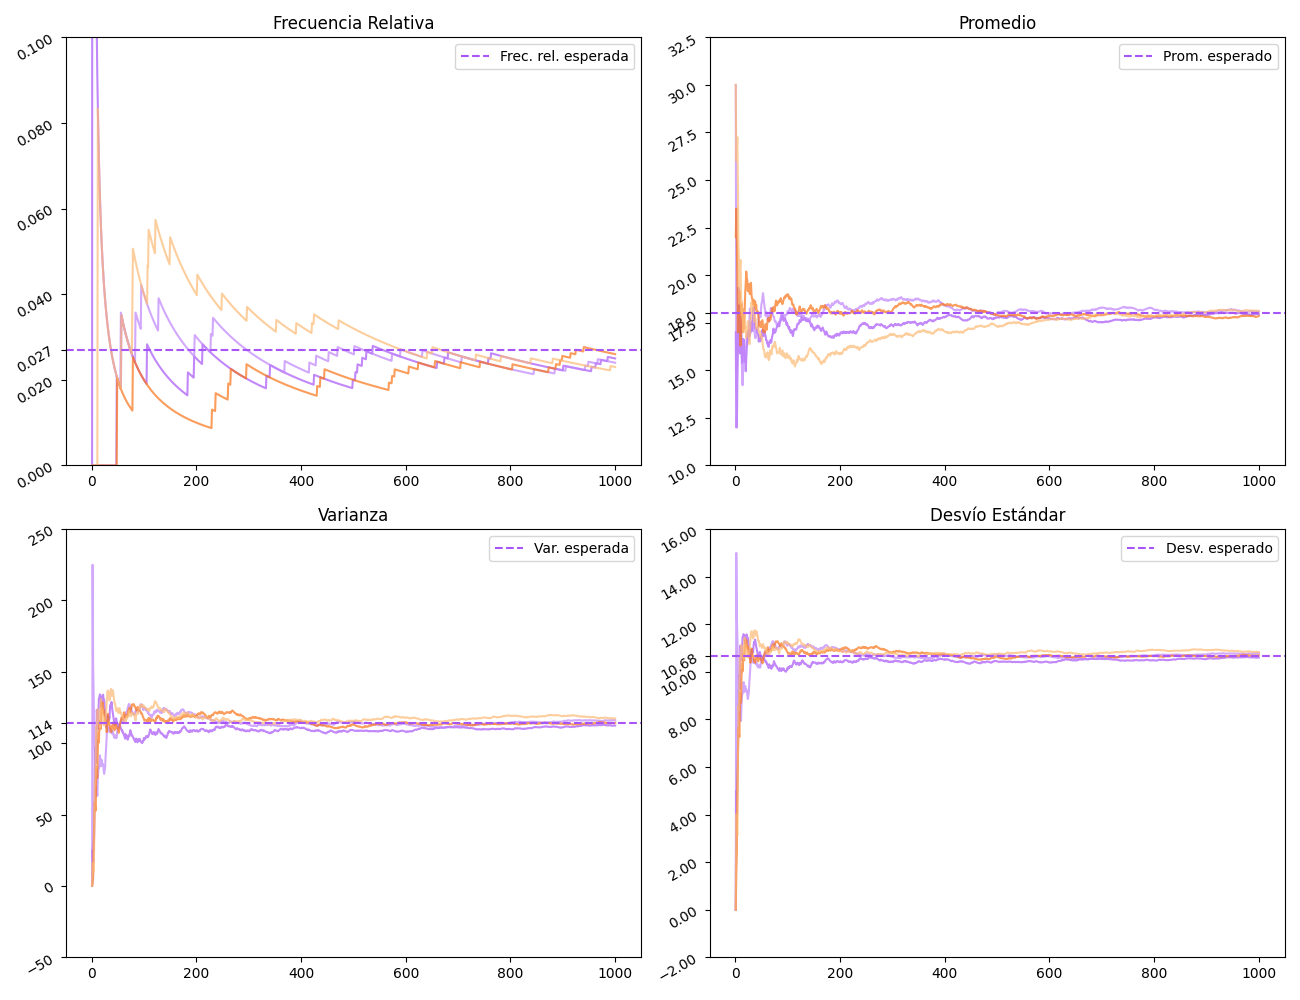
\includegraphics[width=0.8\linewidth]{Imagenes/ParametrosTiradasTotales.png}
    \caption{Parámetros estadísticos de varias corridas}
    \label{fig:parametrosDeTiradas}
\end{figure}

\begin{figure}[H]
    \centering
    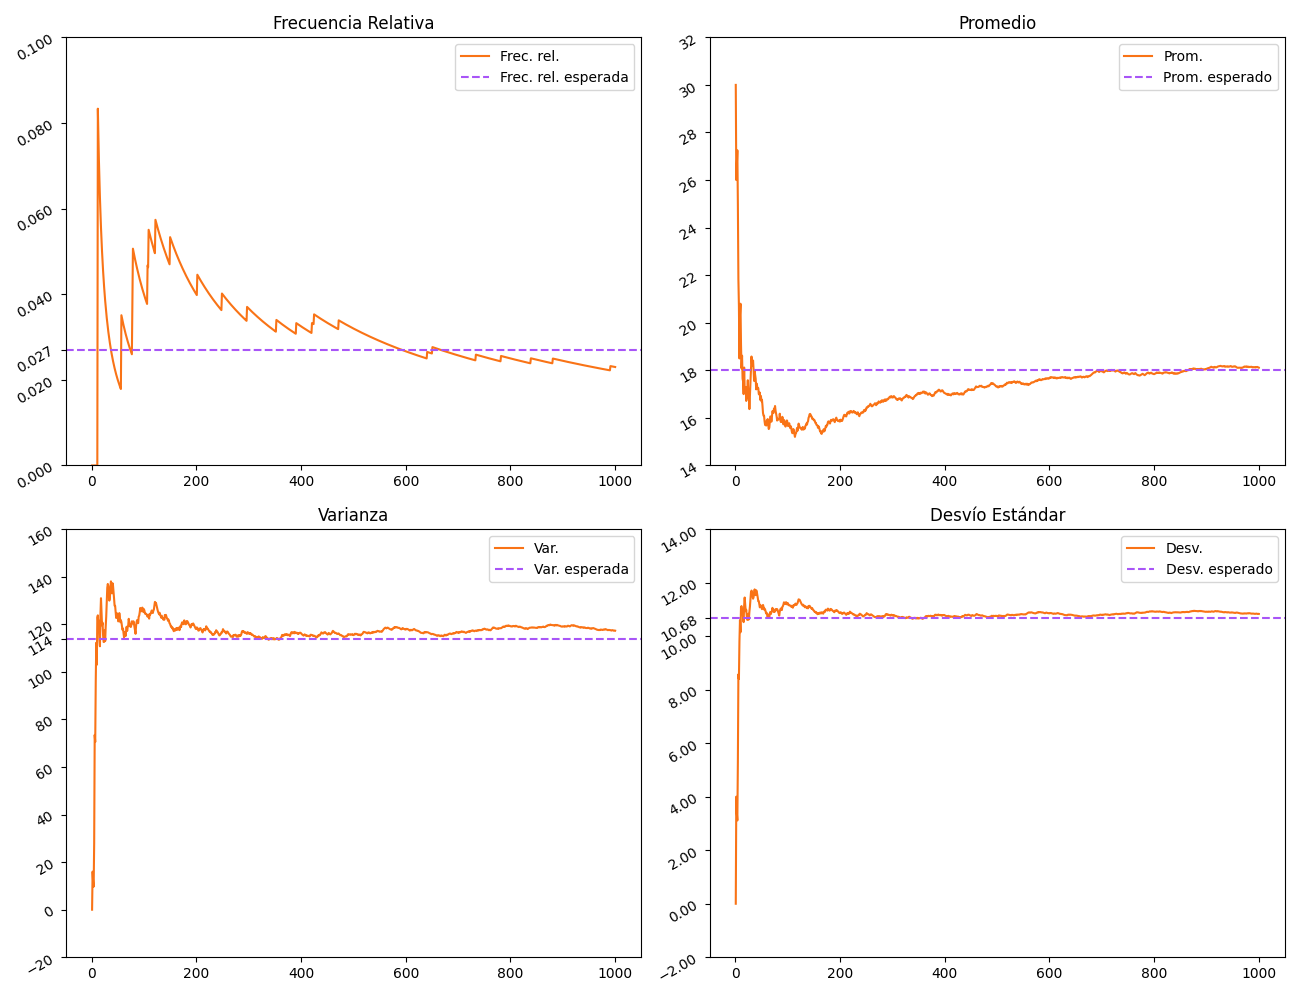
\includegraphics[width=0.8\textwidth]{Imagenes/ParametrosCorrida_4.png}
    \caption{Parámetros estadísticos de una corrida}
    \label{fig:ParametrosCorridas}
\end{figure}

\subsection{Gráficos de Barras} 
\paragraph{Descripción.} 
 Los siguientes gráficos de barras muestran los resultados de cuatro corridas independientes del experimento de simulación, cada una con 1000 tiradas. En cada gráfico se representa la frecuencia absoluta de aparición de los 37 números posibles en una ruleta europea (del 0 al 36).

\paragraph{Análisis Individual.} En cada corrida individual, los números se distribuyen de forma relativamente uniforme, como es esperable en un sistema aleatorio justo. Se observan pequeñas fluctuaciones en la cantidad de apariciones de algunos valores, pero estas no siguen un patrón específico ni sugieren una desviación sistemática.

Estas diferencias responden a la variabilidad natural del azar y tienden a compensarse conforme aumenta el número de tiradas. Así, los graficos de barras individuales muestran cómo la distribución de resultados se aproxima progresivamente a una frecuencia relativa cercana al 2.7\%, que es el valor teórico esperado para cada número. 
\begin{figure}[htbp]
    \centering
    \begin{subfigure}[b]{0.45\textwidth}
        \centering
        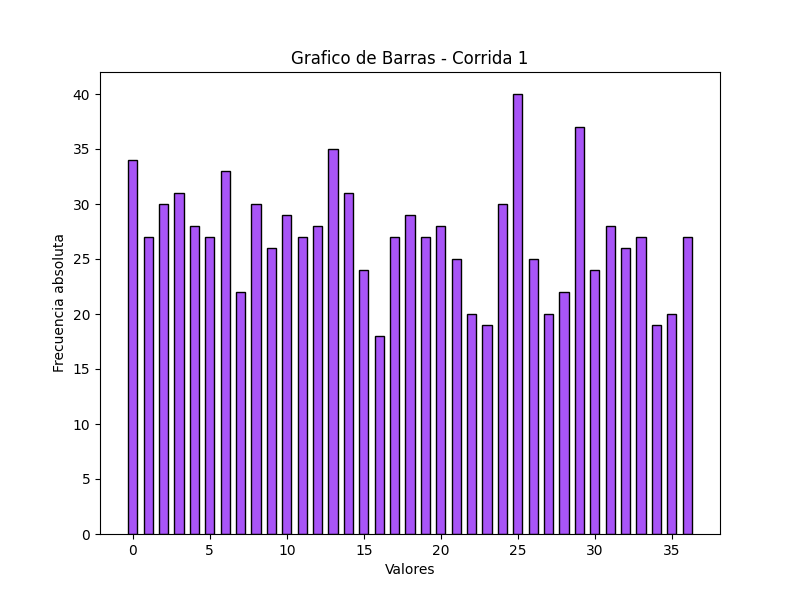
\includegraphics[width=\textwidth]{Imagenes/Barras_corrida_1.png}
        
        \caption{Barras corrida 1}
    \end{subfigure}
    \hfill
    \begin{subfigure}[b]{0.45\textwidth}
        \centering
        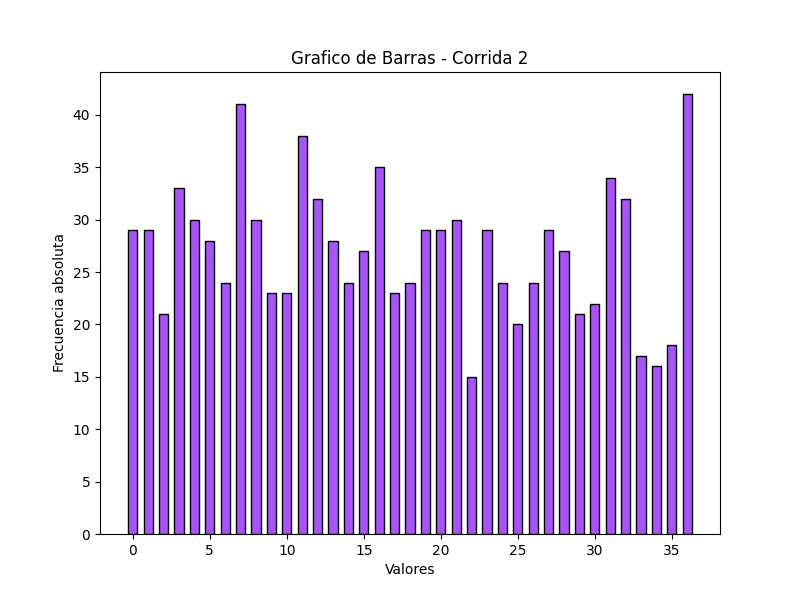
\includegraphics[width=\textwidth]{Imagenes/Barras_corrida_2.png}
        \caption{Barras corrida 2}
    \end{subfigure}
    
    \vspace{0.5cm}
    
    \begin{subfigure}[b]{0.45\textwidth}
        \centering
        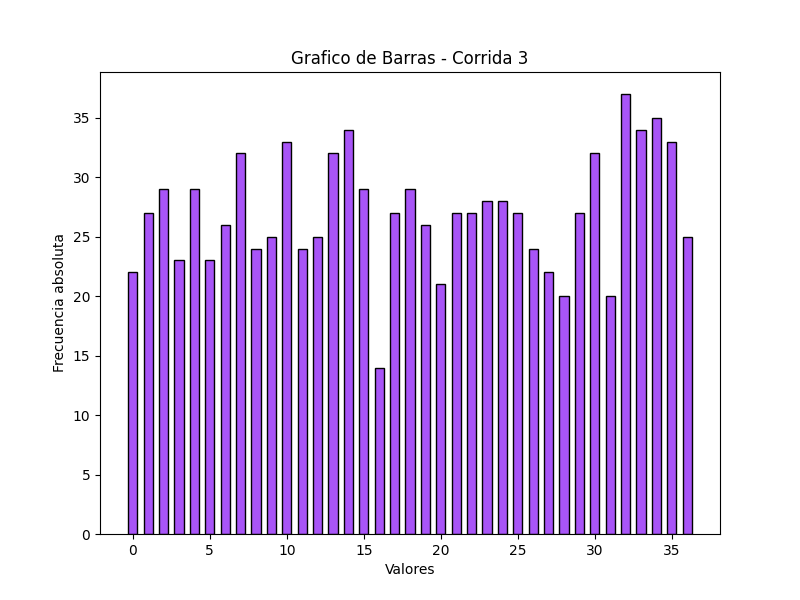
\includegraphics[width=\textwidth]{Imagenes/Barras_corrida_3.png}
        \caption{Barras corrida 3}
    \end{subfigure}
    \hfill
    \begin{subfigure}[b]{0.45\textwidth}
        \centering
        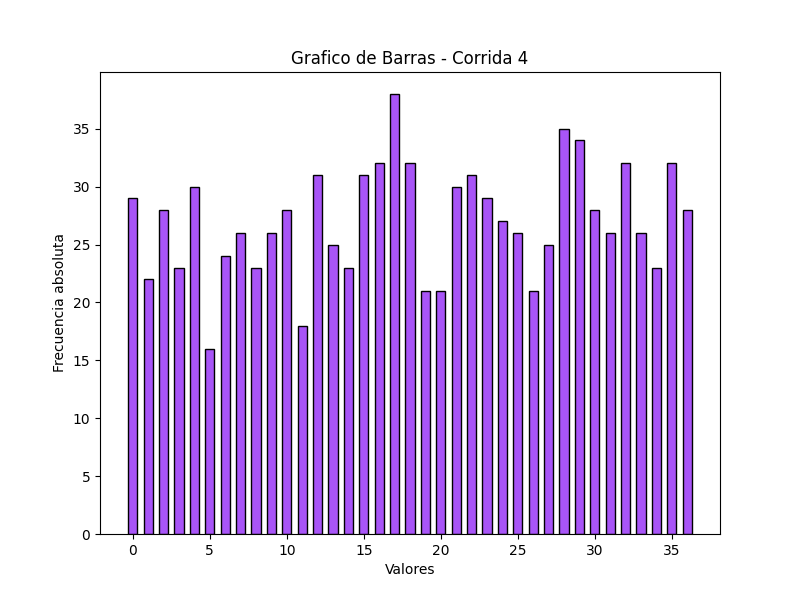
\includegraphics[width=\textwidth]{Imagenes/Barras_corrida_4.png}
        \caption{Barras corrida 4}
    \end{subfigure}

    \caption{Barras individuales por corrida}
    \label{fig:collage}
\end{figure}

\paragraph{Análisis Total.} 
Este gráfico resume la frecuencia absoluta de cada número considerando el total de tiradas acumuladas (4000 en total, producto de las cuatro corridas de 1000 tiradas).

La distribución general de frecuencias es más uniforme que en los gráficos individuales. Las diferencias entre los valores se reducen y se alinean con la distribución teórica de una ruleta justa.
 
Este resultado ejemplifica claramente la Ley de los Grandes Números, que establece que al aumentar la cantidad de repeticiones de un experimento aleatorio, las frecuencias relativas tienden a estabilizarse en torno a sus valores teóricos. En este caso, cada número tiene una probabilidad de aparición cercana a $\frac{1}{37}\approx 2.7\%$, lo cual se refleja empíricamente en el gráfico.
\begin{figure} [H]
    \centering
    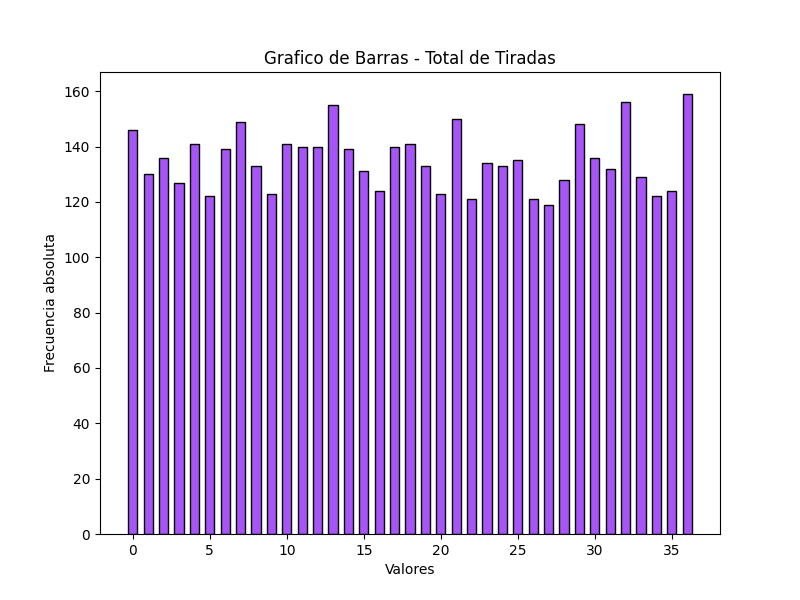
\includegraphics[width=0.5\textwidth]{Imagenes/BarrasTiradasTotales.png}
    \caption{Barras total acumulado}
\end{figure}

\subsection{Distribución por docenas}
\paragraph{Descripción.}
  El siguiente gráfico de torta agrupa los resultados de todas las tiradas según el sistema de docenas utilizado habitualmente en el juego de ruleta. Las categorías son:
    \begin{itemize}
        \item \textbf{Primera Docena:} números del 1 al 12.
        \item \textbf{Segunda Docena:} del 13 al 24.
        \item \textbf{Tercera Docena:} del 25 al 36.
        \item \textbf{Cero:} considerado aparte debido a su rol especial en la ruleta europea. 
    \end{itemize}
Esta organización responde a una forma común de apostar en los casinos, donde cada docena abarca 12 números y tiene una probabilidad teórica de acierto de $\frac{12}{37} \approx 32.43\%$. El cero no pertenece a ninguna docena y representa la ventaja de la casa.
\paragraph{Análisis Total.}
Al considerar la totalidad de las tiradas (4000), el gráfico muestra una distribución más equilibrada y ajustada a las proporciones teóricas. Las tres docenas convergen hacia valores cercanos al 32.43\%, y la aparición del número cero se estabiliza alrededor del 2.7\%.Este resultado confirma nuevamente que el modelo simulado reproduce adecuadamente el comportamiento probabilístico de una ruleta europea real.
 \begin{figure} [htbp]
    \centering
    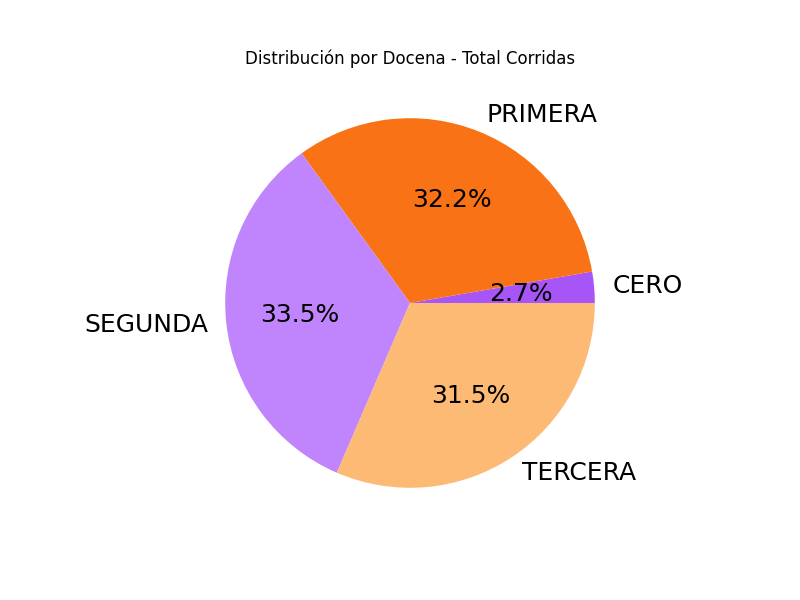
\includegraphics[width=0.5\textwidth]{Imagenes/GraficoTortaTotalCorridas.png}
    \caption{Gráfico de docenas, total corridas}
\end{figure}
\paragraph{Análisis Individual.}
En los gráficos de cada corrida individual, se observa que las tres docenas presentan porcentajes que oscilan en torno al valor teórico esperado. Sin embargo, estas proporciones varían levemente entre corridas, lo cual es coherente con la variabilidad natural del azar. Aun así, no se detectan sesgos significativos ni patrones que indiquen una ruptura de la aleatoriedad: las fluctuaciones son aleatorias y no se concentran en una docena específica.
\begin{figure}[H]
    \centering
    \begin{subfigure}[b]{0.45\textwidth}
        \centering
        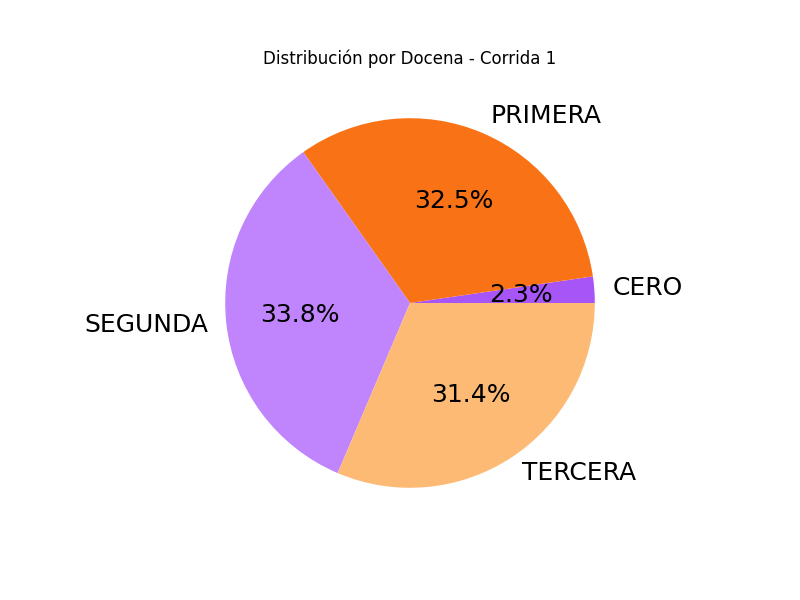
\includegraphics[width=\textwidth]{Imagenes/GraficoTorta_corrida_1.png}
        \caption{Gráfico de docenas, corrida 1}
    \end{subfigure}
    \hfill
    \begin{subfigure}[b]{0.45\textwidth}
        \centering
        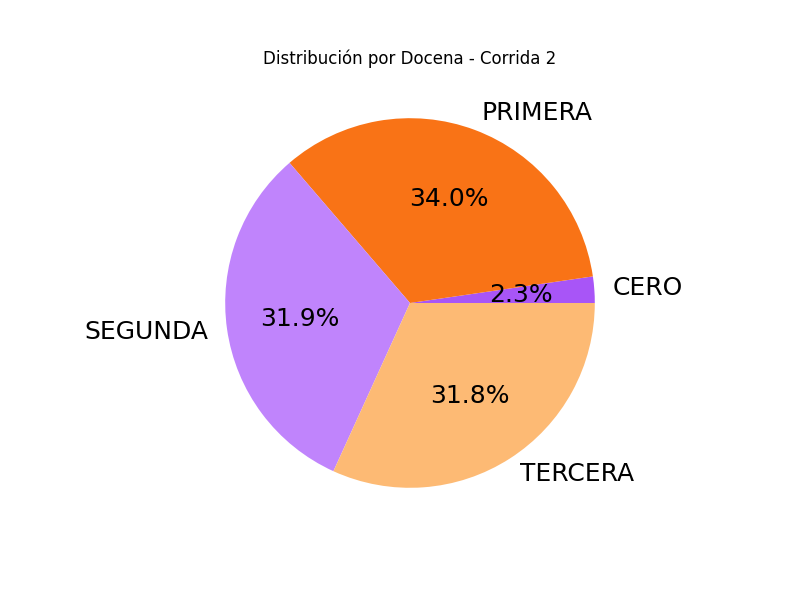
\includegraphics[width=\textwidth]{Imagenes/GraficoTorta_corrida_2.png}
        \caption{Gráfico de docenas, corrida 2}
    \end{subfigure}
    
    \vspace{0.5cm}
    
    \begin{subfigure}[b]{0.45\textwidth}
        \centering
        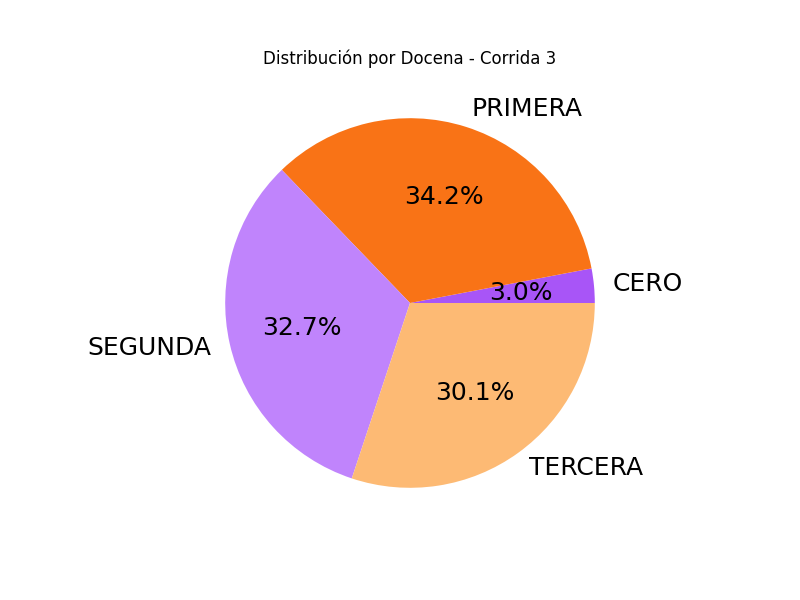
\includegraphics[width=\textwidth]{Imagenes/GraficoTorta_corrida_3.png}
        \caption{Gráfico de docenas, corrida 3}
    \end{subfigure}
    \hfill
    \begin{subfigure}[b]{0.45\textwidth}
        \centering
        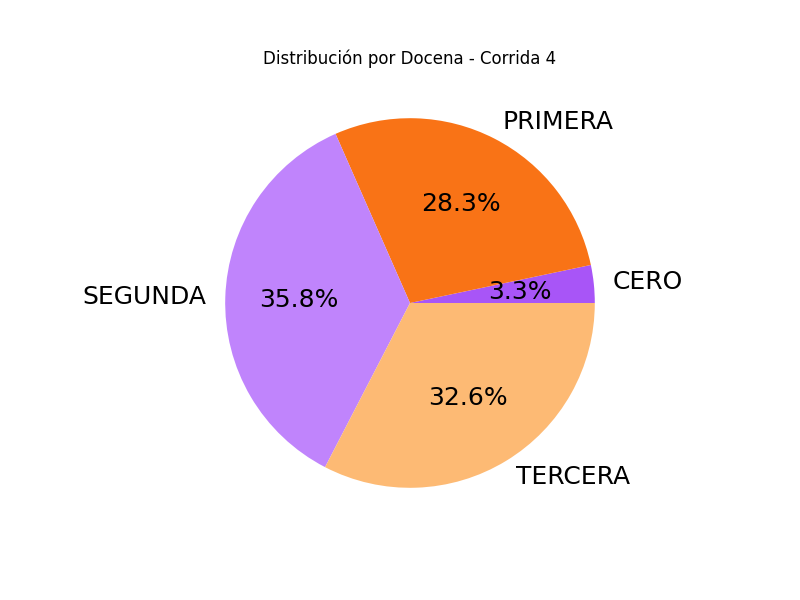
\includegraphics[width=\textwidth]{Imagenes/GraficoTorta_corrida_4.png}
        \caption{Gráfico de docenas, corrida 4}
    \end{subfigure}
    
    \caption{Gráficos de docenas individuales por corrida}
    \label{fig:collage}
\end{figure}

\subsection{Distribución por color}
\paragraph{Descripción.}
Estos gráficos de torta ilustran la distribución porcentual de los resultados según el color de las casillas en la ruleta europea:
    \begin{itemize}
        \item \textbf{Rojo:} 18 números.
        \item \textbf{Negro:} 18 números.
        \item \textbf{Verde:} únicamente el número 0. 
    \end{itemize}

Esta división también forma parte de una modalidad típica de apuestas en ruleta. Los colores rojo y negro presentan una probabilidad teórica de $\frac{18}{37} \approx 48.65\%$, mientras que el verde (el cero) representa una probabilidad de $\frac{1}{37} \approx 2.7\%$.

Este tipo de análisis puede extenderse también a otras clasificaciones clásicas del juego, como par/impar o alto/bajo, que dividen el conjunto de resultados en mitades simétricas con la misma lógica estadística. En todos estos casos, el número cero opera como un elemento de desequilibrio que garantiza la ventaja del casino, ya que no pertenece a ninguno de los grupos apostables.

\paragraph{Análisis Individual.}
En cada corrida individual, se observa un reparto cercano al 50\% entre rojo y negro, con ligeras variaciones atribuibles a la aleatoriedad del experimento. La proporción del color verde, asociada al número cero, es notablemente menor, como se espera teóricamente.
\begin{figure}[H]
    \centering
    \begin{subfigure}[b]{0.45\textwidth}
        \centering
        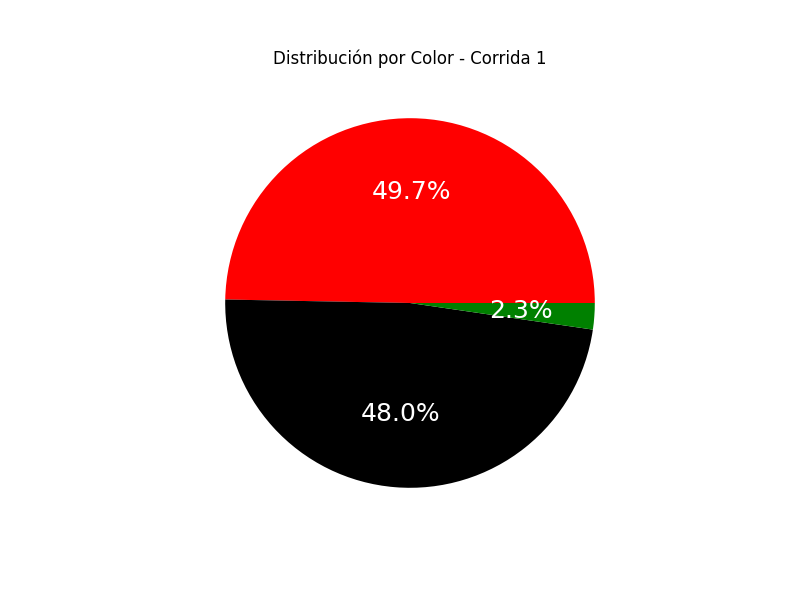
\includegraphics[width=\textwidth]{Imagenes/GraficoColor_corrida_1.png}
        \caption{Gráfico por color, corrida 1}
    \end{subfigure}
    \hfill
    \begin{subfigure}[b]{0.45\textwidth}
        \centering
        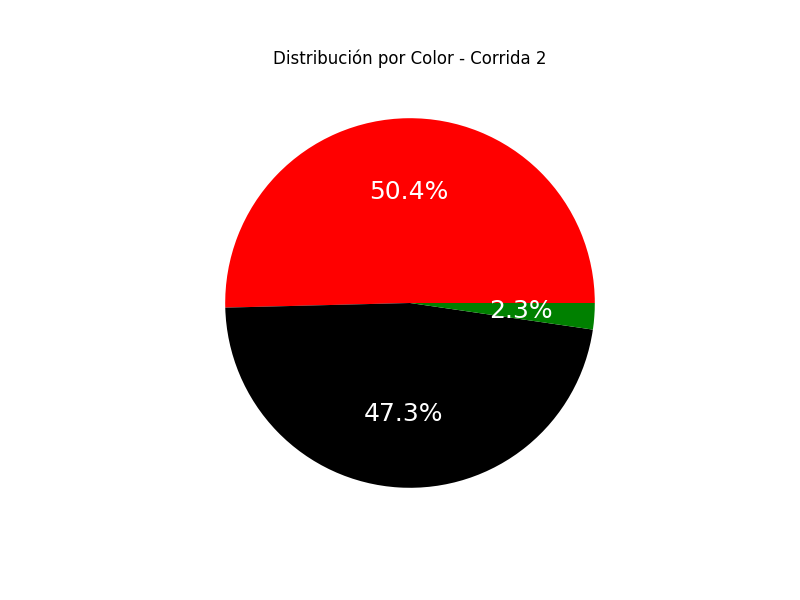
\includegraphics[width=\textwidth]{Imagenes/GraficoColor_corrida_2.png}
        \caption{Gráfico por color, corrida 2}
    \end{subfigure}
    
    \vspace{0.5cm}
    
    \begin{subfigure}[b]{0.45\textwidth}
        \centering
        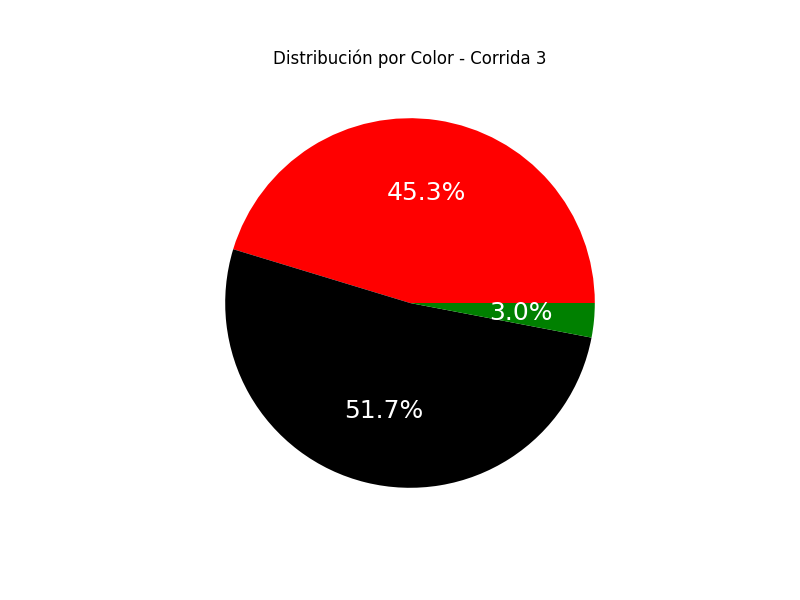
\includegraphics[width=\textwidth]{Imagenes/GraficoColor_corrida_3.png}
        \caption{Gráfico por color, corrida 3}
    \end{subfigure}
    \hfill
    \begin{subfigure}[b]{0.45\textwidth}
        \centering
        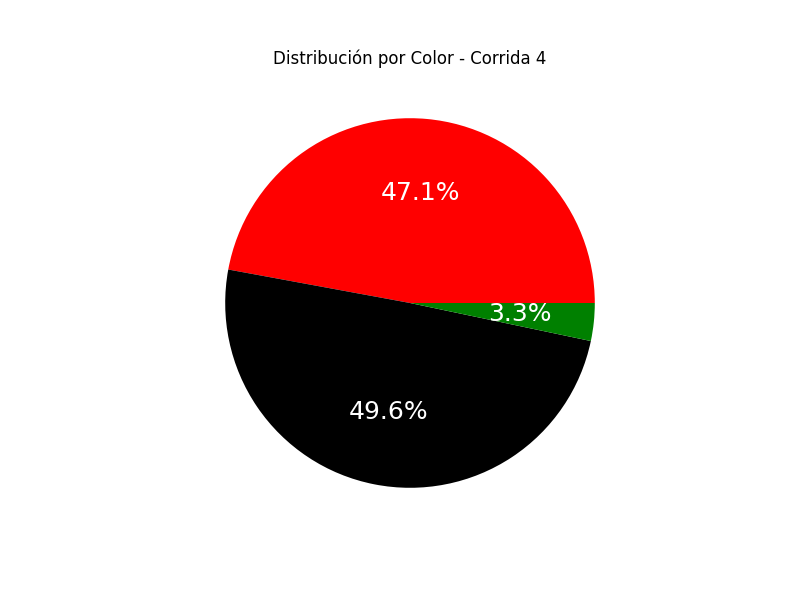
\includegraphics[width=\textwidth]{Imagenes/GraficoColor_corrida_4.png}
        \caption{Gráfico por color, corrida 4}
    \end{subfigure}

    \caption{Gráfico por color individuales por corrida}
    \label{fig:collage}
\end{figure}
\paragraph{Análisis Total.}
Al considerar la totalidad de las tiradas acumuladas, el gráfico general muestra una convergencia aún más clara hacia los valores esperados: rojo y negro tienden a estabilizarse cerca del 48.65\%, mientras que el verde se aproxima al 2.7\%. Esto refuerza la validez del modelo de simulación y su capacidad para reflejar el comportamiento real de una ruleta europea.
\begin{figure} [H]
    \centering
    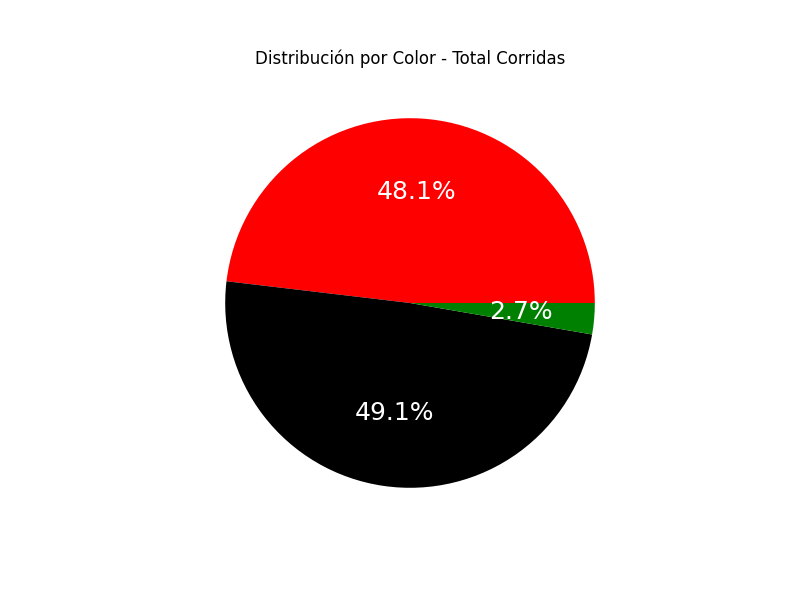
\includegraphics[width=0.5\textwidth]{Imagenes/GraficoColorTotalCorridas.png}
    \caption{Gráfico torta, total corridas}
\end{figure}

\subsection{Ilustración del Teorema Central del Limite}
\par Para demostrar el Teorema Central del Límite, se generaron 500 corridas de 1000 tiradas, se calculó la media de cada corrida y se representaron en un histograma, con una curva de distribución normal (con una media y desvío estándar calculados a partir de estos datos).

\begin{figure} [H]
    \centering
    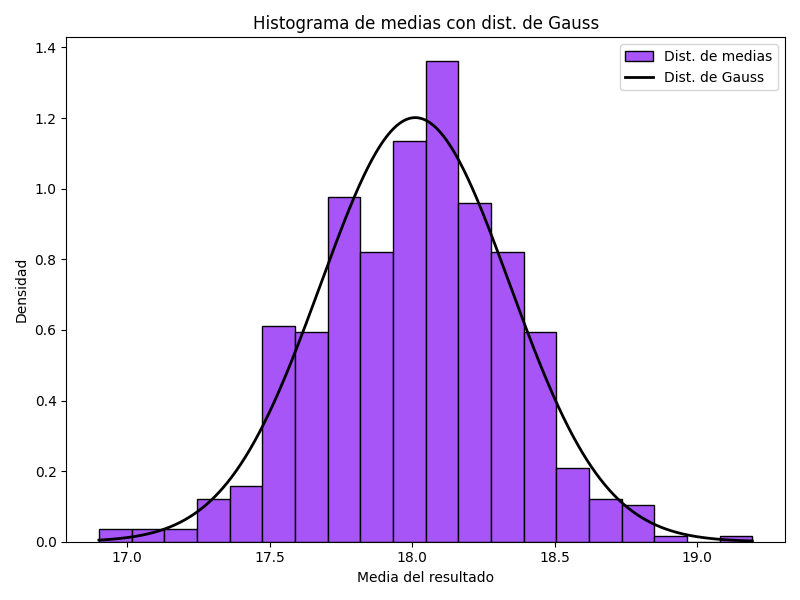
\includegraphics[width=0.5\textwidth]{Imagenes/Histograma_medias_gauss.png}
    \caption{Histograma de medias con distribución de Gauss}
\end{figure}

\paragraph{Análisis.}Esto muestra empíricamente que, aunque la variable original (un entero uniforme de 0 a 36) no sea normal, la distribución de sus medias muestrales tiende a serlo a medida que aumenta el número de observaciones.

\section{Conclusión}
A lo largo de este trabajo se logró simular de forma exitosa el comportamiento estadístico de una ruleta europea mediante técnicas de programación en Python y el uso de herramientas de análisis gráfico. Las simulaciones ejecutadas permitieron contrastar los resultados obtenidos con los valores teóricos esperados, brindando evidencia empírica de fenómenos fundamentales de la estadística, como la Ley de los Grandes Números y el Teorema Central del Límite.

Se observó que, si bien las corridas individuales presentan fluctuaciones en la frecuencia de aparición de los distintos números, estas diferencias tienden a estabilizarse a medida que aumenta la cantidad de tiradas. Este comportamiento es consistente con lo que se espera de un sistema aleatorio justo.

Asimismo, el análisis de las distribuciones por docenas, colores y otros criterios permitió validar que la simulación respeta las proporciones teóricas de la ruleta europea, donde cada número tiene una probabilidad aproximada del 2.7\%, los colores rojo y negro se reparten equitativamente, y el cero introduce la ventaja del casino.

\bibliographystyle{unsrt}  
\begin{thebibliography}{2}

\bibitem{simulaciongithub}
Aldana Risso Patrón. \textit{TP 1.1 - Simulación de una ruleta (código fuente)}.\\
Disponible en: \url{https://github.com/AldanaRP/TPSimulacion} \\

\bibitem{bacchini2018}
Bacchini, H. \textit{Introducción a la Probabilidad y a la Estadística}.\\
Universidad de Buenos Aires, Facultad de Ciencias Económicas, 2018.\\
Disponible en: \url{http://bibliotecadigital.econ.uba.ar/download/libros/Bacchini_Introduccion-a-la-probabilidad-y-a-la-estadistica-2018.pdf}

\end{thebibliography}


\end{document}

